%%%%%%%%%%%%%%%%%%%%%%%%%%%%%%%%%%%%%%%%%%%%%%%%%%%%%%%%%%%%%%%%%
% \documentclass[hyperref={pdfpagelabels=false},compress,table]{beamer} % 在Mac下无法编译
\documentclass[compress,table]{beamer} % 在Mac下使用
% package for font
\usepackage{fontspec}
\defaultfontfeatures{Mapping=tex-text}  %%如果没有它,会有一些 tex 特殊字符无法正常使用,比如连字符。
\usepackage{xunicode,xltxtra}
\usepackage[BoldFont,SlantFont,CJKnumber,CJKchecksingle]{xeCJK}  % \CJKnumber{12345}: 一万二千三百四十五
\usepackage{CJKfntef}  %%实现对汉字加点、下划线等。
\usepackage{pifont}  % \ding{}
% package for math
\usepackage{amsfonts}

% package for graphics
\usepackage[americaninductors,europeanresistors]{circuitikz}
\usepackage{tikz}
\usetikzlibrary{plotmarks}  % placements=positioning
\usepackage{graphicx}  % \includegraphics[]{}
\usepackage{subfigure}  %%图形或表格并排排列
% package for table
\usepackage{colortbl,dcolumn}  %% 彩色表格
\usepackage{multirow}
\usepackage{multicol}
\usepackage{booktabs}
% package for code
\usepackage{fancyvrb}
\usepackage{listings}

% \usepackage{animate}
% \usepackage{movie15}

%%%%%
% setting for beamer
\usetheme{default} % Madrid(常用), Copenhagen, AnnArbor, boxes(白色), Frankfurt,Berkeley
\useoutertheme[subsection=true]{miniframes} % 使用Berkeley时注释本行
\usecolortheme{sidebartab}
\usefonttheme{serif}  %%英文使用衬线字体
% \setbeamertemplate{background canvas}[vertical
% shading][bottom=white,top=structure.fg!7] %%背景色,上25%的蓝,过渡到下白。
\setbeamertemplate{theorems}[numbered]
\setbeamertemplate{navigation symbols}{}  %% 去掉页面下方默认的导航条
\setbeamercovered{transparent}  %设置 beamer 覆盖效果

% 设置标题title背景色
% \setbeamercolor{title}{fg=black, bg=lightgray!60!white}
\setbeamercolor{title}{fg=white, bg=black!70!white}

% 设置每页小LOGO
\pgfdeclareimage[width=1cm]{ouc}{figures/static/ouc.pdf}
\logo{\pgfuseimage{ouc}{\vspace{-20pt}}}

% setting for font
%%\setCJKmainfont{Adobe Kaiti Std}
\setCJKmainfont{SimSun} 
%% \setCJKmainfont{FangSong_GB2312} 
%% \setmainfont{Apple Garamond}  %%苹果字体没有SmallCaps
\setCJKmainfont{SimSun} 
%FUNNY%\setCJKmainfont{DFPShaoNvW5-GB}  %%华康少女文字W5(P)
%FUNNY%\setCJKmainfont{FZJingLeiS-R-GB}  %%方正静蕾体
%FUNNY%\setmainfont{Purisa}
%\setsansfont[Mapping=tex-text]{Adobe Song Std}
     %如果装了Adobe Acrobat,可在font.conf中配置Adobe字体的路径以使用其中文字体。
     %也可直接使用系统中的中文字体如SimSun、SimHei、微软雅黑等。
     %原来beamer用的字体是sans family;注意Mapping的大小写,不能写错。
     %设置字体时也可以直接用字体名,以下三种方式等同:
     %\setromanfont[BoldFont={黑体}]{宋体}
     %\setromanfont[BoldFont={SimHei}]{SimSun}
     %\setromanfont[BoldFont={"[simhei.ttf]"}]{"[simsun.ttc]"}
% setting for graphics
\graphicspath{{figures/}}  %%图片路径
\renewcommand\figurename{图}

% setting for pdf
\hypersetup{% pdfpagemode=FullScreen,%
            pdfauthor={Xiaodong Wang},%
            pdftitle={Title},%
            CJKbookmarks=true,%
            bookmarksnumbered=true,%
            bookmarksopen=false,%
            plainpages=false,%
            colorlinks=true,%
            citecolor=green,%
            filecolor=magenta,%
            linkcolor=blue,%red(default)
            urlcolor=cyan}

% setting for fontspec
\XeTeXlinebreaklocale "zh"  %%表示用中文的断行
\XeTeXlinebreakskip = 0pt plus 1pt minus 0.1pt  %%多一点调整的空间
%%%%%

% font setting by xeCJK
\setCJKfamilyfont{NSimSun}{NSimSun}
\newcommand{\song}{\CJKfamily{NSimSun}}
%%%\setCJKfamilyfont{AdobeSongStd}{Adobe Song Std}
%%%\newcommand{\AdobeSong}{\CJKfamily{AdobeSongStd}}
\setCJKfamilyfont{FangSong}{FangSong_GB2312}
\newcommand{\fang}{\CJKfamily{FangSong}}
%%%\setCJKfamilyfont{AdobeFangsongStd}{Adobe Fangsong Std}
%%%\newcommand{\AdobeFang}{\CJKfamily{AdobeFangsongStd}}
\setCJKfamilyfont{SimHei}{SimHei}
\newcommand{\hei}{\CJKfamily{SimHei}}
%%%\setCJKfamilyfont{AdobeHeitiStd}{Adobe Heiti Std}
%%%\newcommand{\AdobeHei}{\CJKfamily{AdobeHeitiStd}}
\setCJKfamilyfont{KaiTi}{KaiTi}
\newcommand{\kai}{\CJKfamily{KaiTi}}
%%%\setCJKfamilyfont{AdobeKaitiStd}{Adobe Kaiti Std}
\newcommand{\AdobeKai}{\CJKfamily{AdobeKaitiStd}}
\setCJKfamilyfont{LiSu}{LiSu}
\newcommand{\li}{\CJKfamily{LiSu}}
\setCJKfamilyfont{YouYuan}{YouYuan}
\newcommand{\you}{\CJKfamily{YouYuan}}
\setCJKfamilyfont{FZJingLei}{FZJingLeiS-R-GB}
\newcommand{\jinglei}{\CJKfamily{FZJingLei}}
\setCJKfamilyfont{MSYH}{Microsoft YaHei}
\newcommand{\msyh}{\CJKfamily{MSYH}}

% 自定义颜色
\def\Red{\color{red}}
\def\Green{\color{green}}
\def\Blue{\color{blue}}
\def\Mage{\color{magenta}}
\def\Cyan{\color{cyan}}
\def\Brown{\color{brown}}
\def\White{\color{white}}
\def\Black{\color{black}}

\lstnewenvironment{javaCode}[1][]{% for Java
  \lstset{
    basicstyle=\tiny\ttfamily,%
    columns=flexible,%
    framexleftmargin=.7mm, %
    frame=shadowbox,%
    rulesepcolor=\color{cyan},%
    % frame=single,%
    backgroundcolor=\color{white},%
    xleftmargin=4\fboxsep,%
    xrightmargin=4\fboxsep,%
    numbers=left,numberstyle=\tiny,%
    numberblanklines=false,numbersep=7pt,%
    language=Java, %
    }\lstset{#1}}{}

\lstnewenvironment{shCode}[1][]{% for Java
  \lstset{
    basicstyle=\scriptsize\ttfamily,%
    columns=flexible,%
    framexleftmargin=.7mm, %
    frame=shadowbox,%
    rulesepcolor=\color{brown},%
    % frame=single,%
    backgroundcolor=\color{white},%
    xleftmargin=4\fboxsep,%
    xrightmargin=4\fboxsep,%
    numbers=left,numberstyle=\tiny,%
    numberblanklines=false,numbersep=7pt,%
    language=sh, %
    }\lstset{#1}}{}

\newcommand\ask[1]{\vskip 4bp \tikz \node[rectangle,rounded corners,minimum size=6mm,
  fill=white,]{\Cyan \includegraphics[height=1.5cm]{question} \Large \msyh #1};}

\newcommand\wxd[1]{\vskip 4bp \tikz \node[rectangle,minimum size=6mm,
  fill=blue!60!white,]{\White \ding{118} \msyh #1};}

\newcommand\xyy[1]{\vskip 2bp \tikz \node[rectangle,minimum size=3mm,
  fill=black!80!white,]{\White \msyh\scriptsize #1};}

\newcommand\cxf[1]{\vskip 4bp \tikz \node[rectangle,rounded corners,minimum size=6mm,
  fill=orange!60!white,]{\White \ding{42} \msyh #1};}

\newcommand\samp[1]{\vskip 2bp \tikz \node[rectangle,minimum size=3mm,
  fill=white!100!white,]{\Mage\msyh \small CODE \ding{231} \Black #1};\vskip -8bp}

\newcommand\zhyfly[1]{\tikz \node[rectangle,rounded corners,minimum size=6mm,ball
  color=red!25!blue,text=white,]{#1};}

\newcommand\pno[1]{\tikz \node[rectangle,rounded corners,minimum size=1mm,
  fill=yellow!50!black,text=white,]{\msyh\scriptsize P. #1};}

\setbeamerfont{frametitle}{series=\msyh} % 修改Beamer标题字体

\makeatletter
\newcommand{\Extend}[5]{\ext@arrow 0099{\arrowfill@#1#2#3}{#4}{#5}}
\makeatother
%%%%%%%%%%%%%%%%%%%%%%%%%%%%%%%%%%%%%%%%%%%%%%%%
% \titlepage
\title[KevinW@OUC]{\hei {\huge Java 应用程序设计}\\  
  集合与映射}
\author[王晓东]{王晓东\\
  \href{mailto:wxd2870@163.com}{\footnotesize wxd2870@163.com}}
\institute[中国海洋大学]{\small 中国海洋大学}
\date{\today}
\titlegraphic{\vspace{-6em}
\includegraphics[height=6cm]{static/ouc.pdf}\vspace{-6em}}
%%%%%
\begin{document}
%% Delete this, if you do not want the table of contents to pop up at
%% the beginning of each subsection:
\AtBeginSection[]{                              % 在每个Section前都会加入的Frame
  \frame<handout:0>{
    \frametitle{\textbf{\hei 接下来…}}
    \tableofcontents[currentsection]
  }
}  %

\AtBeginSubsection[]                            % 在每个子段落之前
{
  \frame<handout:0>                             % handout:0 表示只在手稿中出现
  {
    \frametitle{\textit{\hei 接下来…}}\small
    \tableofcontents[current,currentsubsection] % 显示在目录中加亮的当前章节
  }
}
 \frame{\titlepage}

%%%%%%%%%%%%%%%%%%%%%%%%%%%%%%%%%%%%%%%%%%%%%%%%
\begin{frame}
\frametitle{参考书目}
\begin{enumerate}
\item 张利国、刘伟[编著], Java SE应用程序设计, 北京理工大学出版社, 2007.10.

\end{enumerate}  
\end{frame}

\begin{frame}
\frametitle{本章学习目标}
\begin{enumerate}
\item 列表(List)
\item 集(Set)
\item 映射(Map)
\item 其它相关API
\end{enumerate}  
\end{frame}

\section*{大纲}
\frame{\frametitle{大纲} \tableofcontents }

\section{集合框架概述}
\begin{frame}[fragile] % [fragile]参数使得能够插入代码
\frametitle{集合框架概述}

集合就是将若干用途、性质相同或相近的“数据”组合而成一个整体。从体系上讲,集合类型可以归纳
为三种:
\begin{description}
\item[集] Set集合中不区分元素的顺序,不允许出现重复元素。例如应用于记录所有用户名的场合。
\item[列表] List集合区分元素的顺序,且允许包含重复元素。相当于数据结构中的线性表,具体表现为数组和向量、链表、栈、队列等。
\item[映射] Map中保存成对的“键 -- 值”(Key -- Value)信息,映射中不能包含重复的键,每个键最多只能映射一个值。
\end{description}

{\Blue\hei Java集合中只能保存引用类型的数据,实际上存放的是对象的引用而非对象本身。Java API中的集合类型均定义在java.util包中。}
\end{frame}

\begin{frame}[fragile] % [fragile]参数使得能够插入代码
\frametitle{集合相关API关系结构}

 \begin{figure}
 \centering
 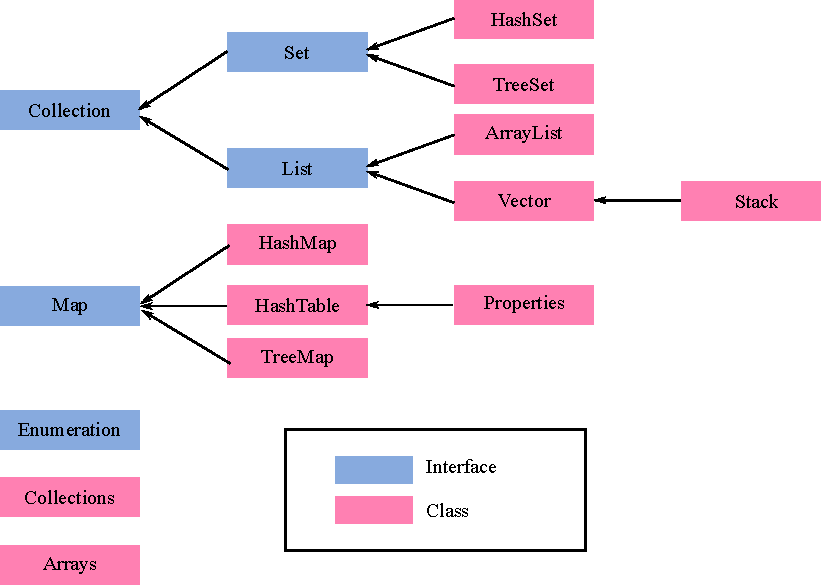
\includegraphics[width=0.8\textwidth]{fig01.pdf}
 \end{figure}
\end{frame}


\section{Collection及Map接口}

\begin{frame}[fragile] % [fragile]参数使得能够插入代码
\frametitle{Collection接口}

java.util.Collection接口是描述Set和List集合类型(不包含Map)的根接口,其中定义了有关集合操作的普遍性方法:
\begin{itemize}[<+-| alert@+>]
\item boolean add(Object o)\\
\only<1>{向集合中添加一个元素,在子接口中此方法发生了分化,如Set接口中添加重复元素时会被拒绝(返回false,而不是出错);List接口则会接受重复元素且返回true。}
\item boolean remove(Object o) \\
\only<2>{从集合中移除指定的元素。}
\item int size()\\
\only<3>{返回集合中元素的数目。}
\item boolean isEmpty()\\
\only<4>{判断集合是否为空(即是否包含任何元素)。}
\item boolean contains(Object o) \\
\only<5>{判断集合中是否包含指定的元素。}
\item void clear()\\
\only<6>{移除当前集合中的所有元素。}
\item Iterator iterator()\\
\only<7>{返回在此集合的元素上进行迭代的迭代器。}
\item Object[] toArray()\\
\only<8>{返回包含当前集合中所有元素的数组。}
\end{itemize}
\end{frame}

\begin{frame}[fragile] % [fragile]参数使得能够插入代码
\frametitle{Set和List接口}

java.util.Set和java.util.List分别描述前述的集和列表结构,二者均为Collection的子接口。

Set接口模拟了数学意义的集合。

List接口规定使用者可以对列表元素的插入位置进行精确控制,并添加了根据元素索引来访问元素等功能,接口中新添加了相应方法:

\begin{itemize}[<+-| alert@+>]
\item void add(int index, Object element)
\item Object get(int index)
\item Object set(int index, Object element) 
\item int indexOf(Object o) 返回列表中首次出现指定元素的索引,如果列表不包含指定元素,则返回-1。
\item Object remove(int index)
\end{itemize}
\end{frame}

\begin{frame}[fragile] % [fragile]参数使得能够插入代码
\frametitle{Map接口}

java.util.Map接口描述了映射结构,Map结构允许以键集、值集合或键—值映射关系集的形式查看某个映射的内容。
主要方法:
\begin{itemize}[<+-| alert@+>]
\item Object put(Object key, Object value)\\
\only<1>{向当前映射中加入一组新的健—值对,并返回所加入元素的“值”,如果此映射中以前包含一个该键的映射关系,则用新值替换旧值。}
\item Object get(Object key)\\
\only<2>{返回此映射中映射到指定键的值,没有则返回null。}
\item boolean isEmpty()
\item void clear()
\item int size()
\item boolean containsKey(Object key)\\
\only<6>{如果映射中包含指定键的映射关系,则返回true,否则返回false。}
\item boolean containsValue(Object value)
\item Set keySet()\\
\only<8>{返回此映射中包含的键的set视图,此Set受映射支持,所以对映射的改变可以在此Set中反映出来,反之亦然。}
\item Collection values()\\
\only<9>{返回此映射包含值的Collection视图,此Collection受映射支持,所以对映射的改变可以在此Collection中反映出来,反之亦然。}
\end{itemize}
\end{frame}

\section{列表}

\begin{frame}[fragile] % [fragile]参数使得能够插入代码
\frametitle{ArrayList类}

java.util.ArrayList类实现了List接口,用于表述长度可变的数组列表。

ArrayList列表允许元素取值为null。除实现了List接口定义的所有功能外,还提供了一些方法来操作列表容量的大小,相关方法包括:

\begin{itemize}
\item public ArrayList()\\构造方法:创建一个初始容量为10的空列表。
\item public ArrayList(int initialCapacity)
\item public void ensureCapacity(int minCapacity)
\item public void trimToSize() \\将此ArrayList实例的容量调整为列表的当前大小。
\end{itemize}
\end{frame}

\begin{frame}[fragile] % [fragile]参数使得能够插入代码
\frametitle{Vector类}

java.util.Vector也实现了List接口,其描述的也是可变长度的对象数组。

\wxd{与ArrayList的差别}

Vector是同步(线程安全)的,运行效率要低一些,主要用在在多线程环境中,而ArrayList是不同步的,适合在单线程环境中使用。

常用方法(除实现List接口中定义的方法外):
\begin{itemize}
\item public Vector()
\item public Object elementAt(int index)
\item public void addElement(Object obj)
\item public void removeElementAt(int index)
\item public void insertElementAt(E obj, int index) 
\item public boolean removeElement(Object obj) 
\item public void removeAllElements()
\item public Object[] toArray()
\end{itemize}
\end{frame}

\begin{frame}[fragile] % [fragile]参数使得能够插入代码
\frametitle{Stack}
java.util.Stack类继承了Vector类,对应数据结构中以“后进先出”(Last in First out, LIFO)方式存储和操作数据的对象栈。
Stack类提供了常规的栈操作方法:
\begin{itemize}
\item public Stack() 构造方法,创建一个空栈。
\item public Object push(E item) 向栈中压入数据。
\item public Object pop() 移除栈顶对象并作为此方法的返回值。
\item public Object peek() 查看/返回栈顶对象,但不从栈中移除它。
\item public boolean empty() 测试栈是否为空。
\item public void clear() 清空栈。
\item public int search(Object o) 返回对象在栈中的位置,以1为基数。
\end{itemize}
\end{frame}

\section{Iterator接口}

\begin{frame}[fragile] % [fragile]参数使得能够插入代码
\frametitle{Iterator接口}

对于ArrayList可以使用get()方法访问其元素,而对于Vector,还可以使用elmentAt()方法访问其元素,后续Set和Map集合也有各自不同的元素访问方式。

{\Blue\hei 是否有一种统一的方式来遍历各种不同类型集合中的元素呢?}\pause

\end{frame}

\begin{frame}[fragile] % [fragile]参数使得能够插入代码
\frametitle{Iterator接口}

Java.util.Iterator接口描述的是以统一方式对各种集合元素进行遍历/迭代的工具,也称为“迭代器”。

迭代器允许在遍历过程中移除集合中的(当前遍历到的那个)元素。主要方法包括:

\begin{itemize}
\item boolean hasNext()\\
如果仍有元素可以迭代,则返回true,否则返回false。
\item Object next()\\
返回迭代的下一个元素,重复调用此方法直到haseNext()方法返回false。
\item void remove()\\
将当前迭代到的元素从迭代器指向的集合中移除。
\end{itemize}
\end{frame}

\begin{frame}[fragile] % [fragile]参数使得能够插入代码
\frametitle{使用迭代器}

我们一般不直接创建迭代器对象,而是通过调用集合对象的iterator()方法(该方法在Collection接口中定义)来获取。

\samp{TestIterator.java}

\begin{javaCode}
import java.util.ArrayList;
import java.util.Iterator;

public class TestIterator {
  public static void main(String[] args) {
    ArrayList a = new ArrayList();
    a.add("China");
    a.add("USA");
    a.add("Korea");
    Iterator it = a.iterator();
    
    while(it.hasNext()) {
      String country = (String) it.next();
      System.out.println(country);
    }
  }
}
\end{javaCode}
{\kai\Red 注意:迭代器相当于原始集合的一个“视图”,即一种表现形式,而不是复制其中所有元素得到的拷贝,因此在迭代器上的操作将影响到原来的集合。}
\end{frame}

\section{集}

\begin{frame}[fragile] % [fragile]参数使得能够插入代码
\frametitle{HashSet类}

java.util.HashSet类实现了java.util.Set接口,描述典型的Set集合结构。

\begin{itemize}
\item HashSet中不允许出现重复元素,不保证集合中元素的顺序。
\item HashSet中允许包含值为null的元素,但最多只能有一个null元素。
\end{itemize}
\end{frame}

\begin{frame}[fragile] % [fragile]参数使得能够插入代码
\frametitle{TreeSet类}

java.util.TreeSet类也实现了java.util.Set,它描述的是Set的一种变体——可以实现排序功能的集合。

在将对象元素添加到TreeSet集中时会自动按照某种比较规则将其插入到有序的对象序列中,以保证TreeSet集合元素组成的对象序列时刻按照“升序”排列(后续介绍升序,例如按照字典顺序排列),对于用户自定义类型的数据我们可以自行定义其所需的排序规则。
\end{frame}

\begin{frame}[fragile] % [fragile]参数使得能够插入代码
\frametitle{Comparable接口}

java.lang.Comparable接口中定义的compareTo()方法用于提供对其实现类的对象进行整体排序所需的比较逻辑,所为的排序可以理解为按照某种标准来比较对象的大小,以确定其次序。
\begin{itemize}\kai
\item 实现类基于compareTo()方法的排序被称为自然排序。而compareTo()方法被称为它的自然比较方法,具体的排序原则可由实现类根据需要而定。方法格式如下:
\begin{verbatim}
int compareTo(Object o)  
\end{verbatim}

\end{itemize}
\end{frame}

\begin{frame}[fragile] % [fragile]参数使得能够插入代码
\frametitle{Comparable接口}

\wxd{使用Comparable接口实现自然排序}
\samp{Person.java}
\begin{javaCode}
public class Person implements java.lang.Comparable {
  private final int id;
  ...

  public Person(int id, String name, int age) {
    this.id = id;
    ...
  }
  ...
  @Override
  public int compareTo(Object o) {
    Person p = (Person) o;
    return this.id - p.id;
  }
  @Override
  public boolean equals(Object o) {
    boolean flag = false;
    if (o instanceof Person) {
      if (this.id == ((Person) o).id) {
        flag = true;
      }
    }
    return false;
  }
} 
\end{javaCode}
\end{frame}

\begin{frame}[fragile] % [fragile]参数使得能够插入代码
\frametitle{Comparable接口}

\samp{TestComparable.java}

\begin{javaCode}
import java.util.TreeSet;
import java.util.Iterator;

public class TestComparable {
  public void static main(String[] args) {
    TreeSet ts = new TreeSet();
    ts.add(new Person(1003, "Bob", 15));
    ts.add(new Person(1008, "Alice", 25));
    ts.add(new Person(1001, "Kevin", 30));
  }
  Iterator it = ts.getIterator();
  while (it.hasNext()) {
    Person emplyee  = (Person) it.next();
    System.out.println(employee);
  }
}
\end{javaCode}

\begin{stdoutCode}
Id: 1001 Name: Kevin Age:30
Id: 1003 Name: Bob Age:15
Id: 1008 Name: Alice Age:25
\end{stdoutCode}
\end{frame}

\begin{frame}[fragile] % [fragile]参数使得能够插入代码
\frametitle{Comparable接口}

\wxd{对上述程序的几点说明}

\begin{enumerate}
\item 用户在重写compareTo()方法以定制比较逻辑时,需要确保其与等价性判断方法equals()保持一致,即确保条件“(x.compareTo(y) == 0) == (x.equals(y))”永远成立,否则逻辑上不合理。所以上例同时重写了equals()方法。
\item 为保证能够实现元素的排序功能,TreeSet集合要求向其加入的对象元素必须是Comparable接口的实现类的实例,否者程序运行时会抛出造型异常(java.lang.ClassCastException)。
\item Comparable接口并不专用于集合框架。
\end{enumerate}
\end{frame}

\section{映射}

\begin{frame}[fragile] % [fragile]参数使得能够插入代码
\frametitle{HashMap类}

java.util.HashMap类实现了java.util.Map接口,该类基于哈希表实现了前述的映射集合结构。
\begin{itemize}
\item HashMap结构不保证其中元素(映射信息)的先后顺序,且允许使用null“值”和null“键”。
\item 当集合中不存在当前检索的“键”所对应的映射值时,HashMap的get()方法会返回空值null,而不会运行出错。
\item 影响HashMap性能的两个参数:初始容量(Initial Capacity)和加载因子(Load Factor)。
\end{itemize}
\end{frame}

\begin{frame}[fragile] % [fragile]参数使得能够插入代码
\frametitle{HashTable类}

java.util.Hashtable与HashMap作用基本相同,也实现了Map接口,采用哈希表的方式将“键”映射到相应的“值”。

\wxd{Hashtable与HashMap的差别}
\begin{itemize}
\item Hashtable中元素的“键”和“值”均不允许为null,而HashMap则允许。
\item Hashtable是同步的,即线程安全的,效率相对要低一些,适合在多线程环境下使用;而 HashMap是不同步的,效率相对高一些,提倡在单线程环境中使用。
\item 除此之外,Hashtable与HashMap的用法格式完全相同。
\end{itemize}
\end{frame}

\begin{frame}[fragile] % [fragile]参数使得能够插入代码
\frametitle{TreeMap类}

java.util.TreeMap类实现了将Map映射中的元素按照“键”进行升序排列的功能,其排序规则可以是默
认的按照“键”的自然顺序排列,也可以使用指定的其他排序规则。

向TreeMap映射中添加的元素“键”所属的类必须实现Comparable接口。

\begin{javaCode}
public MyKey implements Comparable {
  private final int id;
  ...
  public MyKey(int id) {
    this.id = id;
  }
  ...
  @Override
  public int compareTo(Object o) {
    return this.id - ((MyKey) o).id;
  }
  @Override
  public boolean equals(Object o) {
    return (o instanceof MyKey) && (this.id == ((MyKey) o).id);
  }
  @Override
  public int hashCode() {
    return new Integer(id).hasCode();
  }
}  
\end{javaCode}
\end{frame}

\begin{frame}[fragile] % [fragile]参数使得能够插入代码
\frametitle{TreeMap类}
\wxd{对上述程序的说明}

{\kai MyKey类重写equals()方法的同时也重写了hasCode()方法,这是一种规范的做法,目的是为了维护hasCode()方法的常规协定,该协定要求相等对象必须具有相等的哈希码,即当两个对象使用equals()方法比较结果为等价时,它们各自调用hasCode()方法也应该返回相同的结果。}
\end{frame}

\section{其他相关API}
\begin{frame}[fragile] % [fragile]参数使得能够插入代码
  \frametitle{Enumeration接口}

  \xyy{java.util.Enumeration} 接口作用与Iterator接口类似,但只提供了遍
  历Vector和Hashtable(及子类Properties)类型集合元素的功能,且不支持集
  合元素的移除操作。

  \begin{javaCode}
    import java.util.*;

    public class TestEnumeration {
      public static void main(String[] args) {
        Vector v = new Vector();
        v.addElement("Lisa");
        v.addElement("Billy");
        v.addElement("Brown");

        Enumeration e = v.elements();

        while(e.hasMoreElements()) {
          String value = (String) e.nextElement();
          System.out.println(value);
        }
      }
    }
  \end{javaCode}
\end{frame}

\begin{frame}[fragile] % [fragile]参数使得能够插入代码
  \frametitle{Collections类}

  \xyy{java.util.Collections} 类定义了多种集合操作方法,能够实现了对集
  合元素的排序、取极值、批量拷贝、集合结构转换、循环移位以及匹配性检查
  等功能。Collections类的主要方法包括:

  \begin{itemize}
  \item public static void sort(List list)
  \item public static void reverse(List list)
  \item public static void shuffle(List list)
  \item public static void copy(List dest, List src)
  \item public static ArrayList list(Enumeration e)
  \item public static int frequency(Collection c, Object o)
  \item public static T max(Collection coll)
  \item public static T min(Collection coll)
  \item public static void rotate(List list, int distance)
  \end{itemize}
\end{frame}

\begin{frame}[fragile] % [fragile]参数使得能够插入代码
  \frametitle{Arrays类}

  \xyy{java.util.Arrays} 类定义了多种数组操作方法,实现了对数组元素的排
  序、填充、转换为列表或字符串形式、增强的检索和深度比较等功
  能。Arrays类的主要方法包括\footnote{自行搜索学习各方法的用法}:

  \begin{itemize}
  \item public static List asList(Object... a)
  \item public static void sort(<类型>[ ] a)
  \item public static int binarySearch(int[] a, int key)
  \item public static String toString(int[] a)
  \end{itemize}
\end{frame}
%%%%%%%%%%%%%%%%%%%%%%%%%%

%%%%%%%%%%%%%%%%%%%%%%%%%%
%% \begin{frame}
%% \frametitle{本章习题}
%% \begin{enumerate}
%% \item a
%% \item b
%% \end{enumerate}
%% \end{frame}

%% \begin{figure}
%% \centering
%% 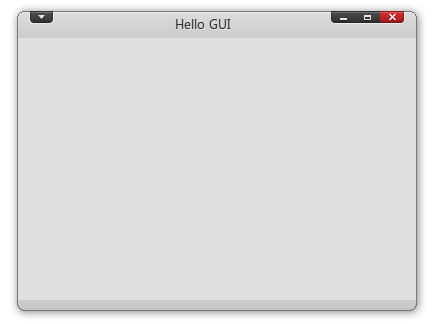
\includegraphics[width=0.6\textwidth]{fig01.png}
%% \end{figure}
% TKS %%%%%%%%%%%%%%%%%%%%%%%%%%%%%%%%%%%%%%%%%%%%%%
\begin{frame}
\centering
{\Huge \textcolor{blue}{THE END}} \\
\vspace{5mm}
{\Large wxd2870@163.com} \\
\end{frame}
%%%%%%%%%%%%%%%%%%%%%%%%%%%%%%%%%%%%%%%%%%%%%%%%%%
\end{document}
